\documentclass[main.tex]{subfiles}
\begin{document}

\section{ Лекция 2. Основные свойства САУ и законы управления }

\subsection{ Задачи управления }

\begin{enumerate}
	\item Достижение заданного состояния: задачи позиционирования (пример: посадка ракеты -- нужно точно приземлиться)
	\item Поддержание заданных параметров, к примеру, задачи стабилизации (например, летит самолёт, надо поддерживать скорость, курс, высоту)
	\item Отслеживание параметров (реализуется в т. н. следящих системах).
	Пример: в катере между штурвалом и рулём посредник -- следящая система, которая позволяет многократно увеличивать усилие (примерно как гидроусилители руля в автомобиле).
	\item Задачи оптимального управления: строим функционал и минимизируем его. Самый высокоразвитый уровень управления: управление наилучшим образом.
\end{enumerate}

\subsection{Качество управления}

Для приведённых выше задач вводим критерий качества $ J $.

\begin{enumerate}[noitemsep]
	\item $J= ||\vec e(T)|| $ -- ошибка в конечный момент времени; $ e = y_\alpha - y $ (ошибка между желаемым и реальным выходом), $ t \in [0;T] $.

    $ y $ -- вектор; пример: при посадке ракеты $ y $ включает координату и скорость.
	\item Поддержание заданных параметров: $ J =||e_{\text{уст}}|| $ - установившаяся ошибка
	\item Отслеживание входных параметров: может быть функционал $ J = \max || e(t) || $
	\item Оптимальное управление: как правило, суммируем какие-то затраты на отдельных участках $ \Rightarrow $ интеграл $ J = \int_{0}^{T}(q ||e(t)||^2 +  \sigma||u||^2)$ ($ e, u $ -- тоже векторы; $ u $ --  управление, $ e $ -- ошибка;  коэффициенты нужны для приведения к одной размерности).

    Энергия -- часто какая-то квадратичная форма ($ \frac{CU^2}{2}, \frac{mv^2}{2} $)
\end{enumerate}

Уменьшение ошибки ведёт, как правило, к увеличению стоимости системы.
Поэтому приходится искать компромисс (и включать кроме ошибки в функционал ограничение на управление).

\subsection{Принципы управления}

\begin{enumerate}[noitemsep]
	\item \emph{Программное управление} -- простейшее. Управляя, не имея модель объекта, нельзя, поэтому считаем, что известна зависимость $ y = f(u, w) $. Предположим, что мы можем обратить зависимость: $ u = \phi(y, w) $ (возмущение $ w $ знаем и оно постоянно, $ y $ задано), т. о. можем найти программно необходимое $ u_{\text{прогр}}(t) $

	\textbf{Пример.}
	Во время Второй мировой войны самолёты сбивали с помощью программного управления (зенитные пушки с неуправляемыми ракетами).
	Но эффективность чрезвычайно низка (управление без обратной связи): лётчик может сделать манёвр.

	Иногда в очень простых системах применять можно.
	\item \emph{Управление по возмущению} -- примерно то же, что программное.
	Предполагаем, что мы можем приблизительно знать и учитывать $ W $ (к примеру, знаем распределение ветров в течение года).

    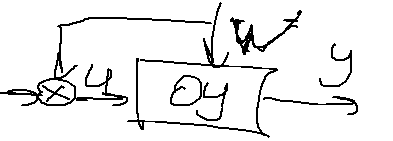
\includegraphics[width=.4\linewidth]{lec2/00_disturb}

	\item \emph{Управление с обратной связью} (ОС): измеряем выходную величину датчиками. Измеренное значение $ y $ поступает в регулятор (управляющее устройство -- УУ), и туда же мы подаём желаемое значение выхода $ y_d $.

    Значение ошибки $ e = y_d - y $ из УУ поступает в исполнительное устройство ИУ, которое формирует управляющий сигнал $ u $.

    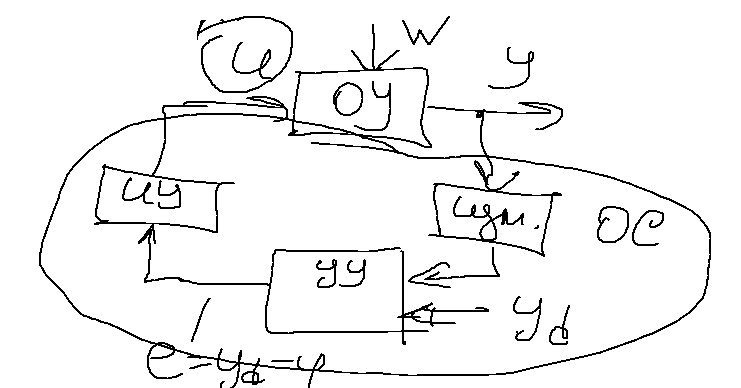
\includegraphics[width=.6\linewidth]{lec2/01_backref}
\end{enumerate}

Какие виды управления мы рассматриваем?

\begin{enumerate}[noitemsep]
	\item Пропорциональный закон управления (p-регулятор): $ u = k_1 e $ -- управление пропорционально ошибке.
	\item Интегральный закон управления: $ u = k_2 \int_{0}^{t} e(\tau)d\tau \longrightarrow (e  \to 0) $

	Этот закон уменьшает накопленную ошибку (интеграл от константной ошибки возрастает $ \Rightarrow $ управление возрастает).
	\item Дифференциальный закон управления: $ u = k_3 \dot e $

	Смысл: уменьшаются колебания ошибки (в предыдущих случаях ошибка может быть небольшой, но колебаться с высокой частотой, как на рисунке внизу).

    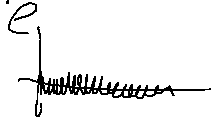
\includegraphics[width=.3\linewidth]{lec2/02_d_reg}

	\item Естественно, может быть комбинация: $ u = k_1e + k_2 \int_{0}^{t} e(\tau)d\tau + k_3 \dot e $ -- \emph{ПИД-регулятор} (пропорционально-интегрально-дифференциальный регулятор) (может быть и \emph{ПИ-регулятор}).

    \item \emph{ Адаптивный регулятор}.

    Пример: днище корабля со временем обрастает моллюсками $ \Rightarrow $ растёт сопротивление.
    Коэффициенты для сопротивления, включённые в модель управления, должны быть подправлены.

    Для этого подаём несколько тестовых сигналов $ u_i $; измеряем выход $ y_i $; вычисляем новые параметры модели.

\end{enumerate}

посмотрим на примере эти законы

\subsubsection{Задача о нагреве тела в ёмкости}

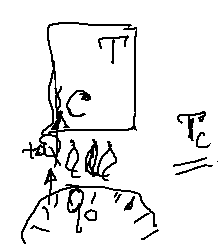
\includegraphics[width=.3\linewidth]{lec2/03_heat}

Пусть имеется некое тело (например, чайник), который надо нагреть ( $T_0 \to T^*$; есть горелка с некой интенсивностью подводимого тепла $ q_0 $).
К примеру, $ T_0=20, T^*=100 $. Пусть тело имеет некую полную теплоёмкость $ C $.

\begin{enumerate}
	\item Подведённая энергия: $ C \Delta T = q_0 \Delta t $ -- баланс энергии.

	Переходим к ДУ: $ C \dot T = q_0 \xrightarrow{q_0 = const} T(t) \xrightarrow[t \to \infty]{} \infty $

	В этой модели мы не учитываем теплоотдачу.

	\item Пусть температура окружающей среды постоянна ($ T_{\text{ср}} = const $)
	$$ C \dot T = q_0 + q_T $$
	Закон Ньютона для теплопередачи: Стефана-Больцмана -- $ E \sim T^4 $ (в кельвинах)

    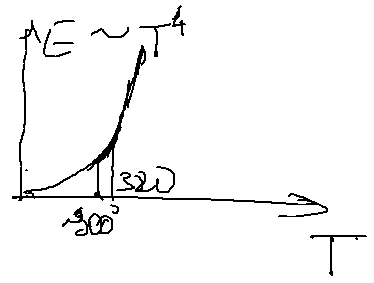
\includegraphics[width=.4\linewidth]{lec2/05_heat_program}

    Закон Ньютона -- его линеаризация в области $ T \approx 300-380 K $: $ q_T = - \alpha(T - T_c) $.
	\begin{align*}
		& C\dot T = q_0 - \alpha (T - T_c) \\
		& T(t) = Ae^{-\frac{\alpha}{C}t} + T_c + \frac{q_0}{\alpha} \xrightarrow{t \to \infty} T_c + \frac{q_0}{\alpha} = T \\
	\end{align*}

    здесь $ \alpha $ -- коэффициент, который зависит от формы, от черноты тела; $ A $ -- некая константа, значение которой нам не так важно.

    Т. о. нашли программное управление

    \[ q_0^{\text{ прогр }} = \alpha (T^* - T_c) \]

    \begin{leftbar}
        Можно тот же закон получить на школьном уровне: при $ t \to \infty $ установившийся процесс $ \Rightarrow $
        сколько тепла приходит в единицу времени, столько и уходит

        \[ q_0 = \alpha (T^* - T_c) \longrightarrow T \ne T^* \]
    \end{leftbar}

	К сожалению, нам неизвестные точные значения параметров $ \alpha, \thickspace T_c $ -- лишь их оценки $ \bar \alpha $, $ \bar T_c $ $ \Rightarrow $ $ T_\infty \ne T^* $.

	Хотим посмотреть, насколько влияет разница предполагаемого значения и реального.

    В реальной системе:
    \begin{align*}
        & \begin{cases}
            C \dot T = q_0 - \bar \alpha (T - \bar T_c) \\
            q_0^{\text{прогр}} = \alpha (T^* - T_c)
        \end{cases}
         \\
         & C\dot T = \alpha (T^* - T_c) - \overline{\alpha}(T - T_c) \\
         & T(t) = Be^{- \frac{\overline{\alpha}}{C}t} + \frac{\alpha(T^* - T_c) + \overline{\alpha} \overline{T}_c}{\overline{\alpha}} \ne T^* \\
    \end{align*}
    $B$ -- некая константа, в общем случае $ B \ne A $.
    В общем случае $ T(t) \ne T^* $; если $ \alpha = \bar \alpha $, $ T(t) = T^* $.

	Отсюда видим, что программное управление неэффективно (даёт ошибку), причём в случае неустойчивой системы ошибка может нарастать до бесконечности.

	\item Сделаем обратную связь. Предположим, что мы можем измерять $ T $; теперь $ u = k_1 e $ (первый вид управления -- пропорциональный), $ q_0 = q_0^{\text{прогр}} + \Delta q_1 $, где $ \Delta q_1 = - k_1 (T - T^*) $, $ k_1 > 0 $.

    Пусть реальные параметры системы -- $ \bar \alpha $, $ \bar T_c $; предполагаемые -- $ \alpha $, $ T_c $.

    \begin{align*}
        & C \dot T = \alpha (T^* - T_c) - k_1 (T - T^*) - \bar \alpha(T - \bar T_c) \\
        & T(t) = De^{ - \frac{\bar \alpha + k_1}{c}t} \\
    \end{align*}

    $ D $ -- очередная константа, значение которой нам неважно.

    Чем такая экспонента хороша?
    Время переходного процесса при этом меньше, чем при программном управлении; решение стремится к частному быстрее.

    Главный результат: конечно, $ T_{\text{ частн }} \ne T^* $, но $ \boxed{ k_1 \to \infty \Rightarrow T \to T^* } $!

    Побочный эффект: $k_1 \nwarrow \Rightarrow $ ошибка уменьшается, но и устойчивость уменьшается.
    Поэтому в более сложных системах нельзя взять

    \item Попробуем вместо П-регулятора взять ПИ-регулятор: $ \Delta q = \Delta q_1 + \Delta q_2 $

    \[ ] \Delta q_2 = - k_2 \int_{0}^{t} (T(\tau) - T^*) d \tau \]
    \begin{align*}
        & C \dot T = \alpha (T^* - T_c) - k_1 (T - T^*) - \bar \alpha (T - \bar T) - k_2 \int_{0}^{t} (T(\tau) - T^*) d \tau  \\
        & \text{ Интегро-дифференциальное уравнение; решаем дифференцированием: } \\
        & e = T - T^* \Rightarrow \dot e = \dot T, \thickspace \ddot e = \ddot T \\
        & c \ddot e = - k_1 \dot e - \bar \alpha \dot e - k_2 e \\
        & c \ddot e + (\bar \alpha + k_1) \dot e + k_2 e = 0 \\
    \end{align*}

    Получилось уравнение вида
    \[ a \ddot x + b \dot x + cx = 0, \thickspace a, b, c > 0 \]
    В таком уравнении $ x \xrightarrow[t \to \infty]{} 0 $ в нашем уравнении относительно ошибки $ \Rightarrow $ $ e \xrightarrow[t \to \infty]{} 0 \Leftrightarrow T \to T^*  \forall k_1, k_2 > 0 $ (это лучше, чем при пропорциональном управлении).

    Можно обойтись без пропорционального закона?
    Нельзя.
    Если $ \bar \alpha = 0 $, то с одним лишь интегральным регулятором будут незатухающие колебания.

	% TODO всё до второго перерыва пропущено

\end{enumerate}

\subsection{Часть 3 лекции | Структура ТАУ}

ТАУ:

\begin{enumerate}[noitemsep]
	\item Анализ: имеется система; надо выяснить её свойства  (например, чтобы понять, почему плохо работает).
	\item Синтез (конструируем модель системы управления, затем и саму систему) -- обратная задача.
	Зачастую обратная задача решается через многократное решение задач анализа с последующим изменением системы.
\end{enumerate}

\subsubsection{Анализ систем автоматического управления}

\begin{enumerate}[noitemsep]
	\item Построение математической модели (ММ). От адекватности модели зависит эффективность управления.
	\item Анализ установившегося процесса:
	\begin{enumerate}[noitemsep]
		\item \emph{Устойчивость:} все системы должны быть устойчивы.
		Нужно узнавать приближение неустойчивости и уметь с ней бороться.
		\item \emph{Точность:} с какой точностью функционирует наша система, какова величина ошибки управления?
	\end{enumerate}
	\item Анализ переходного процесса (пример: у самолёта это взлёт / посадка, где происходит подавляющее количество аварий).
	Нас при этом интересуют:
	\begin{enumerate}[noitemsep]
		\item Время переходного процесса $ t_{\text{ПП}} $. При перелёте из СПб в Москву, к примеру, после взлёта сразу следует посадка -- установившегося процесса нет, всё время переходный.

		\item Режим этого процесса.

        Возможны три режима: монотонный, апериодический с одним пиком или колебательный.

        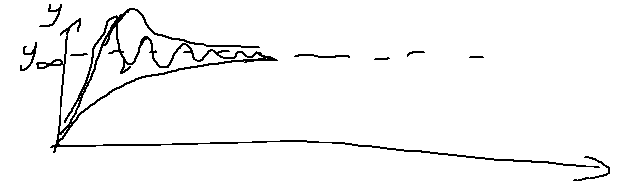
\includegraphics[width=.4\linewidth]{lec2/06_transition}
	\end{enumerate}
\end{enumerate}

\subsubsection{ Какие можно построить математические модели? }

\[ \xrightarrow{u} \overset{\downarrow
    W}{\boxed{\text{ОУ}}}\xrightarrow{y} \]

Если процесс безинерционный (подаём сигнал на вход и мгновенно получаем изменение выхода), к примеру, $ y = au + bw $, алгебраическое уравнение -- \emph{статические} (безинерционные) системы:

Если же в процессах есть инерция, системы называются \emph{динамическими}.
Они описываются не алгебраическими, а дифференциальными уравнениями.

Иногда в разные моменты времени одну и ту же систему можно рассматривать как статическую (например, в установившемся режиме) и как динамическую.

\subsubsection{Основные принципы построения ММ}

Модель, конечно же, лучше всего пытаться разделить на блоки (\textbf{принцип разбиения на более мелкие звенья}).
Но надо помнить: каждое звено должно иметь \emph{однонаправленное действие}, то есть выход звена не влияет на его вход.

Последнее требование позволяет отдельно работать с математической моделью каждого звена.

Как проверить принцип однонаправленности?
Мысленно уберём одно звено (например, ММ2 -- см. рис. ниже).
Если работа предыдущего звена ММ1 не изменится, принцип однонаправленности действия соблюдён.

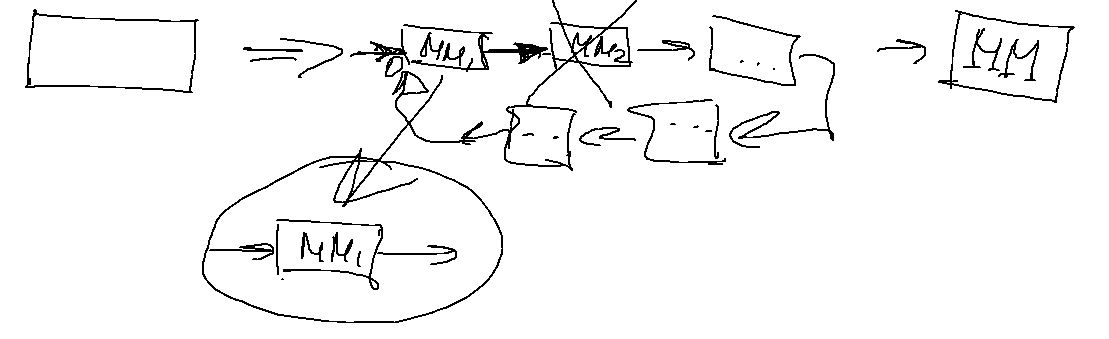
\includegraphics[width=.6\linewidth]{lec2/07_model_principals}

Пример: в автомобиле (в первом приближении) можно выделить спидометр как подсистему, у которой вход не зависит от выхода.

\textbf{Пример: задача}. Рассмотрим катер или автомобиль с электроусилителем руля.

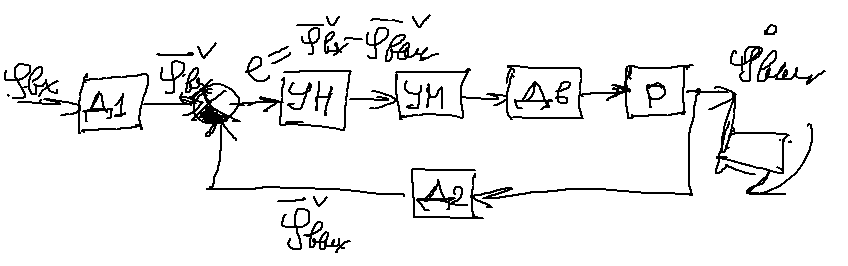
\includegraphics[width=.7\linewidth]{lec2/08_example_steering}

$ \phi_{\text{вход}} $ -- угол поворота руля в данный момент;  $ \phi_{\text{вход}}^V $ -- электрический сигнал, напряжение; УН -- усилитель напряжения, УМ -- усилитель мощность (усилив напряжение, усиливаем ток); ДВ -- двигатель (обычно -- двигатель постоянного тока).
Двигатель обычно работает в пару с Р -- редуктором, который понижает скорость.

После редуктора получаем выходной угол $ \phi_{\text{вых}} $, который измеряется датчиком Д2.
Измеренный датчиком электрический сигнал $ \bar \phi_{\text{вых}}^V $ (точнее, разность $ e = \bar \phi_{\text{вх}}^V - \phi_{\text{вых}}^V $) поступает обратно в УН.


\subsection{Линейные непрерывные стационарные системы (ЛНСС)}

Линейные, т. к. проще: можем получить общие результаты аналитически (выполняется \emph{принцип суперпозиции}: $ \alpha u_1 + \beta u_2 \to \alpha y_1 + \beta y_2 $).

Имея произвольный входной сигнал $ u $, можно найти реакцию от одного малого участка $ u_i \Rightarrow $ этого достаточно!
Воспользовавшись принципом суперпозиции, сдвигая и масштабируя это решение, получим $ y = \sum c_i y_i (t - t_i) $.

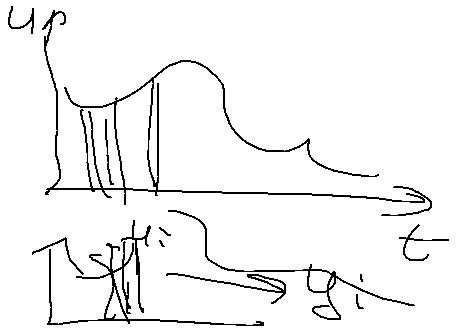
\includegraphics[width=.6\linewidth]{lec2/09_linear_input}

В нелинейном анализе, как правило, можно получить только частные результаты.
Но зато можно иногда применять линейную теорию:

\begin{enumerate}[noitemsep]
    \item Нелинейность на входе иногда можно компенсировать нелинейностью в цепи обратной связи.

    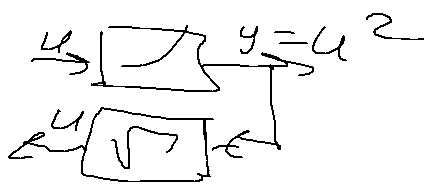
\includegraphics[width=.4\linewidth]{lec2/10_compensation}

    \item Когда нельзя компенсировать нелинейность, прибегаем к \emph{линеаризации}.
\end{enumerate}

Линеаризовать сигнал можно только на маленьком участке.
Пример -- закон Стефана-Больцмана.

Конечно, бывают системы, которые хорошо описываются только нелинейными моделями, но мы такие не рассматриваем.

Итак,
\begin{enumerate}[noitemsep]
	\item Линейные системы: это проще
	\item Непрерывные: в современном мире, конечно, всё чаще дискретные; но, отдавая дань традиции, вначале изучаем непрерывные.
	\item Стационарные системы -- системы с постоянными параметрами (постоянные коэффициенты в уравнениях, например, жёсткость пружины в колебательной системе со временем считаем переменной).
	Ракету нельзя считать стационарной системой: масса меняется.

	\begin{itemize}[noitemsep]
		\item Пример: статическая система: раскладываем в ряд Тейлора $ y = f(u^*, w^*) + \frac{\partial f}{\partial u} |_* \Delta u + \frac{\partial f}{\partial w} |_* \Delta w + ... $

		Слагаемые более высокого порядка отбрасываем (когда вторые производные конечны).
        Здесь $ u^* $ -- точка, в окрестности которой линеаризуем систему.

        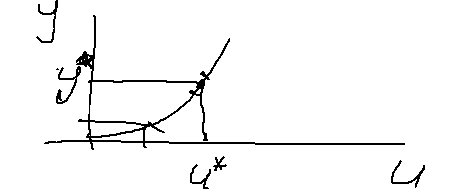
\includegraphics[width=.4\linewidth]{lec2/11_linearization}

        Уравнение в отклонениях:

        \[ \Delta y = a \Delta u + b \Delta w \]

        В номинальном режиме (т. е. вблизи точки, где раскладываем в ряд)

        \[ f^* +  \left. \frac{\partial f}{\partial y}\right|_* \Delta y + \left. \frac{\partial f}{\partial \dot y} \right|_* \dot{\Delta y} + ... = 0 \]

		\item Пример динамической системы: $ f(y, \dot y, \ddot y, u,  \dot u, w) = 0 $

		После линеаризации: $ \alpha_2 \ddot{\Delta y} + \alpha_1 \dot{\Delta y} + \alpha_0 y = \beta_1 \dot{\Delta u} + \beta_0 \Delta u + \gamma_0 w $

		Это уравнение в отклонениях. \emph{Далее будем рассматривать все уравнения в отклонениях и опускать дельты.}
	\end{itemize}

\end{enumerate}

\subsection{Формальное описание ЛНСДС (линейных непрерывных стационарных динамических систем)}

Рассмотрим ДУ порядка $ n $

\begin{equation}\label{eq:linear_de}
    \alpha_n y^{(n)} + ... + \alpha_0 y = \beta_m u^{(m)} + ... + \beta_0 u
\end{equation}

Чтобы однозначно определить решение \eqref{eq:linear_de}, нужно $ n $ начальных условий: $ y(0)=y_0, \dot y(0) = \dot y_0, ... $

$ D \equiv \frac{d}{dt} $ -- оператор дифференцирования.
Тогда

\begin{equation}
	(\alpha_n D^n + ... + \alpha_0) y = (\beta_n D^m + ... + \beta_0) u
\end{equation}

В операторном виде уравнение \eqref{eq:linear_de} выглядит так:
\begin{equation*}
    	\boxed{ \alpha (D) y = \beta(D) u }
\end{equation*}

Определение. $ \alpha(D) $ называют \emph{характеристическим полиномом} системы (в нём заложены основные свойства системы: устойчивость и т. д)., а его степень -- \emph{порядком} системы.

Определение. $ n > m \to $ \emph{строго реализуемая} система -- её можно собрать, спаять...

$ n = m \to $ \emph{нестрого реализуемая} (физическая) система; $ n < m $ -- \emph{нереализуемая} система (такое мы не можем себе позволить).

\textbf{Пример.} Грузик тащим по поверхности, действует сила трения $ F = m \ddot x $. Здесь $ \alpha(D) = mD^2, \beta(D) = 1, n = 2 > m = 0 $ ($ m $ в последнем случае -- порядок $ \beta $, не масса)

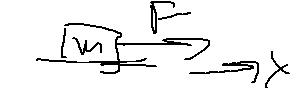
\includegraphics[width=.4\linewidth]{lec2/12_friction}

\textbf{Пример 2.} Грузик, подвешенный на пружине с демпфером:

\[ m \ddot y = - c y - b \dot y + F \Rightarrow \begin{cases}
    \alpha(D) = mD^2 + bD + c \\
    \beta(D) = 1 \\
\end{cases} \]

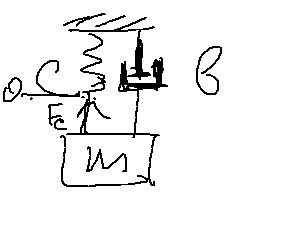
\includegraphics[width=.35\linewidth]{lec2/13_damper}

\textbf{Если на экзамене спрошу: <<а где $ m\vec{g} $?>>, то ответ <<сократилось, мы считаем отклонение от положения равновесия>>}.

\textbf{Пример 3.} Закон Ома для участка цепи:

\[ I = \frac{U}{R} \Rightarrow \begin{cases}
    \alpha = 1 \thickspace (n = 0) \\
    \beta = \frac{1}{R} \thickspace (m=0)
\end{cases} \]

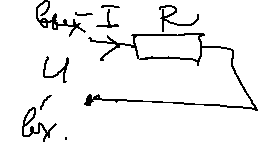
\includegraphics[width=.35\linewidth]{lec2/14_soldering}

Система нестрого реализуемая -- некая идеализация: не учитываем сопротивление проводов.
Давайте учтём.

\textbf{Пример 3а.} Рассматриваем RC-контур.

Ёмкость -- коэффициент пропорциональности между напряжением на обкладках и зарядом: $ dq = C \cdot dU $

Конденсатор -- \emph{реактивное} сопротивление (в отличие от активного сопротивления, на конденсаторе мощность не выделяется): $ \frac{d q}{d t} = C \frac{d U}{d t} \to I = C \cdot DU \to X_c = \frac{1}{CD} $ -- реактивное сопротивление.

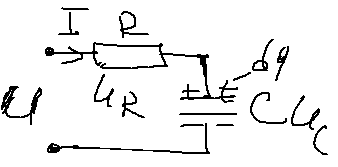
\includegraphics[width=.35\linewidth]{lec2/15_rc}

Падение напряжения: $ \dot U = \dot U_R + \dot U_C $
\begin{align*}
    & DU = R \cdot DI + \frac{I}{C} \\
    & (RCD + 1)I = C \cdot DU \\
    & \begin{cases}
        \alpha(D)  = RCD + 1 \\
        \beta(D) = CD
    \end{cases} \\
\end{align*}

Т. о. теперь $ n = m = 1 $ -- снова нестрого реализуемая система, некая идеализация.

\textbf{ Пример 3а+ }. Что, если просто воткнём в розетку конденсатор?

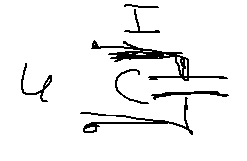
\includegraphics[width=.3\linewidth]{lec2/16_c}

\[ I = C \cdot DU \Rightarrow \begin{cases}
    \alpha(D) = 1 \\
    \beta(D) = 0
\end{cases} \]
$ n = m = 1 \Rightarrow $ система нереализуемая (нельзя не учитывать внутреннее сопротивление конденсатора).

В самом деле, в RC-контуре при $ R \to 0 $ ток в начальный момент $ I(0) \to \infty $.

\textbf{Пример 3б.} Заметим, что в модели 3а в нуле разрыв производной.
Природа не терпит не только бесконечные величины, но и бесконечные производные.
Учитываем индуктивность проводов: RC-контур становится RLC-контуром.

Конденсатор накапливает назад, катушка -- магнитное поле.
Индуктивность катушки -- коэффициент пропорциональности между изменением тока и возникающей ЭДС:
\[ U_L = L =\frac{d I}{d t} \]
Т. о. $ L $ -- реактивное ёмкостное сопротивление.

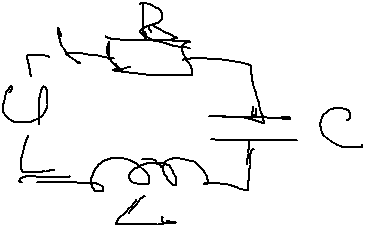
\includegraphics[width=.35\linewidth]{lec2/17_rlc}

\begin{align*}
    & U_L = L \cdot DI \\
    & \dot U = \dot U_R + \dot U_C + \dot U_L \\
    & DU = RDI + \frac{I}{C} + LD^2 I \\
    & (LCD^2 + RCD + 1)I = CDU \\
    & \begin{cases}
        \alpha(D) = LCD^2 + RCD + 1, \thickspace n = 2 \\
        \beta(D) = CD, \thickspace m = 1 < n
    \end{cases}
\end{align*}
Система строго реализуемая!

Зависимость тока от времени: вначале быстро возрастает, но не мгновенно благодаря катушке.

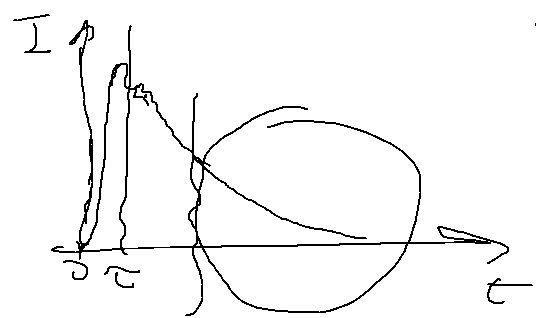
\includegraphics[width=.35\linewidth]{lec2/18_rlc_current}

В области, обведённой кружочком, нас устраивает модель $ RC $. \\

Отступление.
Электрошокер устроен так: батарея + катушка индуктивности; ключ в нормальном режиме замкнут, когда нужно кого-то ударить током, ключ размыкают.
$ U_L = \frac{d I}{d t} $ -- очень большое напряжение.

\end{document}